\documentclass[12pt, a4paper]{book}

\usepackage[T1]{fontenc}
\usepackage[utf8]{inputenc}
\usepackage[charter, cal=cmcal]{mathdesign}
\usepackage[scaled=0.92]{helvet}
\usepackage{geometry}
\geometry{a4paper, top=30mm, bottom=30mm, inner=32mm, outer=25mm, marginparwidth=18mm}

\usepackage{amsmath, amsthm}
\usepackage[version=4]{mhchem}
\usepackage{graphicx}
\usepackage{xcolor}
\usepackage{tikz}
\usetikzlibrary{arrows.meta, shapes.geometric, positioning, calc, backgrounds}
\usepackage{pgfplots}
\pgfplotsset{compat=1.18}
\usepackage{tcolorbox}
\tcbuselibrary{skins, breakable, theorems}
\usepackage{titlesec}
\usepackage{fancyhdr}
\usepackage{enumitem}
\usepackage{booktabs}
\usepackage{array}
\usepackage{parskip}
\usepackage{siunitx}
\usepackage[colorlinks=true, linkcolor=BrickRed,
            urlcolor=NavyBlue, citecolor=ForestGreen]{hyperref}

% ── Colours (Journey 2 — charcoal / royal blue) ────────────────────────────────
\definecolor{JourneyColor}{HTML}{0F172A}
\definecolor{ModuleColor}{HTML}{2563EB}
\definecolor{PuzzleColor}{HTML}{D97706}
\definecolor{DiscoveryColor}{HTML}{3B82F6}
\definecolor{WarningColor}{HTML}{991B1B}
\definecolor{ProblemColor}{HTML}{6B21A8}
\definecolor{ReflectColor}{HTML}{0D9488}
\definecolor{HistoryColor}{HTML}{78350F}

% ── Boxes ─────────────────────────────────────────────────────────────────────
\newtcolorbox{puzzlebox}[1][]{enhanced,breakable,
  colback=PuzzleColor!6,colframe=PuzzleColor,fonttitle=\bfseries\sffamily,
  title={The Puzzle},attach boxed title to top left={yshift=-2mm,xshift=6mm},
  boxed title style={colback=PuzzleColor},borderline west={3pt}{0pt}{PuzzleColor},#1}

\newtcolorbox{discoverybox}[1][]{enhanced,breakable,
  colback=DiscoveryColor!8,colframe=DiscoveryColor,fonttitle=\bfseries\sffamily,
  title={Discovery},attach boxed title to top left={yshift=-2mm,xshift=6mm},
  boxed title style={colback=DiscoveryColor},borderline west={3pt}{0pt}{DiscoveryColor},#1}

\newtcolorbox{problembox}[1][]{enhanced,breakable,
  colback=ProblemColor!5,colframe=ProblemColor,fonttitle=\bfseries\sffamily,
  title={Problems},attach boxed title to top left={yshift=-2mm,xshift=6mm},
  boxed title style={colback=ProblemColor},borderline west={3pt}{0pt}{ProblemColor},#1}

\newtcolorbox{deepbox}[1][]{enhanced,breakable,
  colback=JourneyColor!5,colframe=JourneyColor,fonttitle=\bfseries\sffamily,
  title={Deep Problems},attach boxed title to top left={yshift=-2mm,xshift=6mm},
  boxed title style={colback=JourneyColor},borderline west={4pt}{0pt}{JourneyColor},#1}

\newtcolorbox{historybox}[1][]{enhanced,breakable,
  colback=HistoryColor!7,colframe=HistoryColor!60,fonttitle=\bfseries\sffamily\small,
  title={Historical Note},attach boxed title to top left={yshift=-2mm,xshift=6mm},
  boxed title style={colback=HistoryColor!80},#1}

\newtcolorbox{reflectionbox}[1][]{enhanced,breakable,
  colback=ReflectColor!6,colframe=ReflectColor,fonttitle=\bfseries\sffamily,
  title={Reflection},attach boxed title to top left={yshift=-2mm,xshift=6mm},
  boxed title style={colback=ReflectColor},borderline west={3pt}{0pt}{ReflectColor},#1}

\newtcolorbox{namedconcept}[2][]{enhanced,
  colback=ModuleColor!6,colframe=ModuleColor,fonttitle=\bfseries\sffamily\large,
  title={#2},attach boxed title to top left={yshift=-2mm,xshift=6mm},
  boxed title style={colback=ModuleColor},#1}

% ── Section formatting ────────────────────────────────────────────────────────
\titleformat{\chapter}[display]
  {\normalfont\sffamily\huge\bfseries\color{JourneyColor}}
  {\textcolor{JourneyColor!60}{\chaptertitlename\ \thechapter}}{10pt}{\Huge}
  [\vspace{2pt}\textcolor{JourneyColor}{\titlerule[1.5pt]}]
\titleformat{\section}
  {\normalfont\sffamily\Large\bfseries\color{ModuleColor}}
  {\thesection}{1em}{}[\textcolor{ModuleColor!40}{\titlerule[0.6pt]}]
\titleformat{\subsection}
  {\normalfont\sffamily\large\bfseries\color{JourneyColor!80}}{\thesubsection}{1em}{}
\titleformat{\subsubsection}
  {\normalfont\sffamily\normalsize\bfseries}{\thesubsubsection}{1em}{}

\pagestyle{fancy}
\fancyhf{}
\fancyhead[LE]{\small\sffamily\textcolor{JourneyColor}{\leftmark}}
\fancyhead[RO]{\small\sffamily\textcolor{ModuleColor}{\rightmark}}
\fancyfoot[C]{\small\thepage}
\renewcommand{\headrulewidth}{0.4pt}

\newcommand{\newterm}[1]{\textit{\textcolor{DiscoveryColor}{#1}}}
\newcommand{\important}[1]{\textcolor{ModuleColor}{\textbf{#1}}}

\begin{document}

\setcounter{chapter}{1}
\chapter[Journey 2 --- Physical Computation (Silicon to Gate)]
        {Journey Two\\[8pt]
         \textcolor{ModuleColor}{\large Physical Computation (Silicon to Gate)}}
\setcounter{section}{0}

\section{Module 2.1 --- Transistor Physics and MOSFETs}
\label{sec:mod2.1}

\subsection*{Motivation}

We completed in Journey 1 the abstract theory of information, studying binary representations, entropy limits, and logic.
But computation is not just a mathematical abstraction. It is a physical process.
To construct a physical computer, we must build a physical switch.

Modern computing is built upon the **MOSFET** (Metal-Oxide-Semiconductor Field-Effect Transistor).
A silicon chip contains billions of these microscopic switches.
By applying a voltage to a control contact, we can switch a block of silicon from being a near-perfect insulator to a conductor.
This module bridges physical chemistry and computer engineering.
We will explore the solid-state chemistry of semiconductor doping, the physics of channel formation, and derive the electrical equations that turn silicon into the logical engine of our processors.

\subsection{The Voltage-Controlled Switch}

We analyze how chemical impurities in silicon allow us to control current with an electric field.

\begin{puzzlebox}
\textbf{The Silicon Valve.}

Suppose we want to construct an automatic logical switch.
If we apply a small electric voltage to a control wire, we want another circuit to turn ON (allowing current to flow). If we remove that voltage, we want it to turn OFF (blocking current).
Modern chips use the MOSFET as this switch. It is built on a single crystal of silicon.
\begin{enumerate}[label=(\alph*), leftmargin=*]
  \item Silicon is in Group 14, possessing four valence electrons.
        * **n-type doping:** We replace a fraction of silicon atoms with phosphorus (Group 15, 5 valence electrons).
        * **p-type doping:** We replace a fraction of silicon atoms with boron (Group 13, 3 valence electrons).
        Explain why the extra electron of phosphorus is free to move in the conduction band, whereas the missing electron of boron creates a positive "hole" in the valence band.
  \item An n-channel MOSFET (nMOS) consists of a p-type silicon substrate (body) containing two highly doped n-type regions: the **Source** and the **Drain**.
        A metal contact, the **Gate**, is placed directly above the p-type body between the Source and Drain, separated by a thin insulating layer of silicon dioxide ($\ce{SiO2}$).
        
        If the gate voltage is zero, explain why no current can flow between Source and Drain when a voltage is applied between them. (Hint: Think about the two back-to-back p-n junctions formed).
  \item If we apply a positive voltage to the Gate, it creates an electric field through the $\ce{SiO2}$ layer.
        Explain how this field repels holes in the p-type substrate under the gate and attracts electrons, creating a thin, conducting n-type channel linking the Source to the Drain.
\end{enumerate}
\end{puzzlebox}

\subsection{MOSFET Structure and Inversion}

We model the electrostatic state of the transistor under gate bias.

\begin{center}
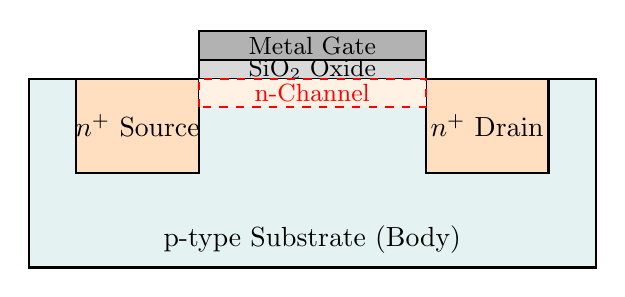
\begin{tikzpicture}[scale=1.2]
  % P-substrate body
  \draw[fill=teal!10, thick] (0,0) rectangle (6,2);
  \node at (3,0.3) {p-type Substrate (Body)};
  
  % Source (n+)
  \draw[fill=orange!25, thick] (0.5,1.0) rectangle (1.8,2.0);
  \node at (1.15,1.5) {$n^+$ Source};
  
  % Drain (n+)
  \draw[fill=orange!25, thick] (4.2,1.0) rectangle (5.5,2.0);
  \node at (4.85,1.5) {$n^+$ Drain};
  
  % Oxide layer (SiO2)
  \draw[fill=gray!30, thick] (1.8,2.0) rectangle (4.2,2.2);
  \node[font=\small] at (3,2.1) {$\ce{SiO2}$ Oxide};
  
  % Gate electrode
  \draw[fill=gray!60, thick] (1.8,2.2) rectangle (4.2,2.5);
  \node[font=\small] at (3,2.35) {Metal Gate};
  
  % Sub-gate channel region (inversion layer)
  \draw[dashed, red, fill=orange!10, thick] (1.8,1.7) rectangle (4.2,2.0);
  \node[red, font=\small] at (3,1.85) {n-Channel};
\end{tikzpicture}
\end{center}

\begin{explobox}
We define the **Threshold Voltage** ($V_{th}$) as the minimum gate-to-source voltage ($V_{GS}$) required to form this conducting channel. This state is called **strong inversion**.
* For $V_{GS} < V_{th}$, the transistor is in **Cutoff** (switch open).
* For $V_{GS} \ge V_{th}$, the channel forms.
  * If the drain-source voltage $V_{DS}$ is small, the current $I_D$ scales linearly with $V_{DS}$ (the **Triode/Linear region**).
  * If $V_{DS}$ is large ($V_{DS} \ge V_{GS} - V_{th}$), the channel pinches off near the drain, and the current saturates, becoming independent of $V_{DS}$ (the **Saturation region**).
\begin{enumerate}[label=(\alph*), leftmargin=*]
  \item Why does the channel pinch off near the drain when $V_{DS}$ is large? (Consider the local voltage difference between the Gate and the channel at the drain edge: $V_{gate} - V_{channel}(L) = V_{GS} - V_{DS}$).
  \item Write down a qualitative plot of the drain current $I_D$ versus $V_{DS}$ for different values of $V_{GS}$. Mark the boundary between triode and saturation regions.
  \item A PMOS transistor is the exact dual of an nMOS: it has an n-type substrate with $p^+$ source/drain regions.
        What polarity of gate-to-source voltage ($V_{GS}$) is required to turn a pMOS transistor ON? (Why must it attract positive holes to form the channel?)
\end{enumerate}
\end{explobox}

\subsection{Transistor Scaling Limits}

We analyze the physical limits of Moore's Law.

\begin{explobox}
For decades, computer performance has doubled every two years by shrinking the physical channel length $L$ of MOSFETs (enabling more transistors to fit on a chip).
Modern process nodes have channel lengths of only a few nanometers.
At these scales, several non-idealities arise:
1. **Short-Channel Effects:** The drain voltage starts to control the channel electrostatic potential directly, lowering the barrier and increasing leakage current even when the gate is turned OFF (Drain-Induced Barrier Lowering, DIBL).
2. **Quantum Tunneling:** The insulating $\ce{SiO2}$ oxide layer becomes so thin ($\le \SI{1.5}{nm}$) that electrons can tunnel directly through it quantum mechanically, causing massive gate leakage currents.
\begin{enumerate}[label=(\alph*), leftmargin=*]
  \item Why does quantum tunneling (from Physics Journey 6 Module 3) represent an absolute physical limit to how thin we can make the gate oxide layer?
  \item If the gate oxide leaks current, how does this affect the power consumption and heat dissipation of a idle computer processor?
\end{enumerate}
\end{explobox}

\newpage

% ─── Section: Discovery ──────────────────────────────────────────────────────
\section{Part 3 --- Discovery}

\begin{discoverybox}
\textbf{What have we built?}

\textbf{First.} Doping silicon with phosphorus (Group 15) or boron (Group 13) introduces free electrons (n-type) or holes (p-type), shifting the material's conductivity.

\textbf{Second.} A MOSFET is a three-terminal voltage-controlled switch: applying a gate voltage $V_{GS}$ above the threshold voltage $V_{th}$ creates an electric field that attracts charge carriers to form an inversion channel between Source and Drain.

\textbf{Third.} Under bias, the MOSFET operates in three regions: Cutoff ($I_D \approx 0$), Triode (linear resistance), and Saturation (constant current after channel pinch-off).

\textbf{Fourth.} Physical scaling of transistors faces fundamental quantum and electrostatic limits: DIBL and gate-oxide quantum tunneling leakage restrict silicon scaling below a few atomic layers.
\end{discoverybox}

\newpage

% ─── Section: Naming Concepts ────────────────────────────────────────────────
\section{Part 4 --- What This Is Called}

\begin{namedconcept}{Transistor Physics parameters}
* **MOSFET:** Metal-Oxide-Semiconductor Field-Effect Transistor. A voltage-controlled solid-state switch.
* **nMOS:** A MOSFET with an n-type channel formed in a p-type substrate.
* **pMOS:** A MOSFET with a p-type channel formed in an n-type substrate.
* **Inversion Layer:** The thin layer of semiconductor under the gate oxide that changes its electrical character (e.g. p-type to n-type) due to gate bias.
* **Threshold Voltage ($V_{th}$):** The minimum gate-source voltage required to form the inversion layer channel.
* **Pinch-Off:** The reduction of channel depth to zero near the drain contact when the drain voltage is high, causing current saturation.
\end{namedconcept}

\newpage

% ─── Section: Solved Exercises ───────────────────────────────────────────────
\section{Part 5 --- Solved Exercises}

\begin{problembox}
\begin{enumerate}[label=\textbf{E\arabic*.}]
  \item \textbf{Calculating Gate Oxide Capacitance.}
  
        Prove that the gate capacitance per unit area of a MOSFET is $C_{ox} = \frac{\epsilon_{ox}}{t_{ox}}$, where $\epsilon_{ox} = \epsilon_r \epsilon_0$ is the permittivity of the oxide insulator and $t_{ox}$ is the oxide thickness.
        Calculate the value of $C_{ox}$ (in F/m$^2$ and fF/$\mu$m$^2$) for a modern processor with oxide thickness $t_{ox} = \SI{1.5}{nm}$ and relative permittivity of silicon dioxide $\epsilon_r = 3.9$.
        
        \textbf{Solution:}
        A MOSFET gate can be modeled as a parallel-plate capacitor.
        The capacitance $C$ of a parallel-plate capacitor is:
        \[
          C \;=\; \frac{\epsilon A}{d}.
        \]
        Here, the insulator permittivity is $\epsilon = \epsilon_{ox}$, the area is $A$, and the distance is the oxide thickness $d = t_{ox}$.
        The capacitance per unit area $C_{ox} = C / A$ is:
        \[
          C_{ox} \;=\; \frac{\epsilon_{ox}}{t_{ox}}.
        \]
        This completes the proof.
        
        Now, substitute the values to calculate $C_{ox}$:
        * $\epsilon_0 \approx 8.854 \times 10^{-12}$ F/m (permittivity of free space).
        * $\epsilon_r = 3.9 \implies \epsilon_{ox} = 3.9 \times 8.854 \times 10^{-12}$ F/m $= 3.453 \times 10^{-11}$ F/m.
        * $t_{ox} = \SI{1.5}{nm} = 1.5 \times 10^{-9}$ m.
        
        \[
          C_{ox} \;=\; \frac{3.453 \times 10^{-11} \text{ F/m}}{1.5 \times 10^{-9} \text{ m}} \;=\; 2.30 \times 10^{-2} \text{ F/m}^2.
        \]
        To convert to fF/$\mu$m$^2$:
        * $1 \text{ F} = 10^{15} \text{ fF}$.
        * $1 \text{ m}^2 = 10^{12} \text{ }\mu\text{m}^2$.
        \[
          C_{ox} \;=\; 2.30 \times 10^{-2} \times \frac{10^{15} \text{ fF}}{10^{12} \text{ }\mu\text{m}^2} \;=\; 23.0 \text{ fF/}\mu\text{m}^2.
        \]
        Thus, the capacitance per unit area is $\SI{2.30 \times 10^{-2}}{F/m^2}$ or $\SI{23.0}{fF/\mu m^2}$.
        
  \item \textbf{Dopant Concentration and Silicon Resistivity.}
  
        To construct the $n^+$ source/drain regions, silicon is doped with phosphorus.
        The electrical conductivity of n-type silicon is given by $\sigma = q N_D \mu_n$, where $q = 1.602 \times 10^{-19}$ C is the electron charge, $N_D$ is the donor dopant concentration, and $\mu_n \approx \SI{1350}{cm^2/V\cdot s}$ is the electron mobility.
        Calculate the donor concentration $N_D$ (in cm$^{-3}$) required to achieve a resistivity of $\rho = \SI{0.1}{\Omega\cdot cm}$.
        
        \textbf{Solution:}
        By definition, resistivity $\rho$ is the reciprocal of conductivity:
        \[
          \rho \;=\; \frac{1}{\sigma} \;=\; \frac{1}{q N_D \mu_n}.
        \]
        Solve this equation for the donor concentration $N_D$:
        \[
          N_D \;=\; \frac{1}{q \rho \mu_n}.
        \]
        Substitute the given values:
        * $\rho = \SI{0.1}{\Omega\cdot cm}$.
        * $\mu_n = \SI{1350}{cm^2/V\cdot s}$.
        * $q = 1.602 \times 10^{-19}$ C.
        
        \[
          N_D \;=\; \frac{1}{\left( 1.602 \times 10^{-19} \text{ C} \right) \left( 0.1 \;\Omega\cdot\text{cm} \right) \left( 1350 \text{ cm}^2/\text{V}\cdot\text{s} \right)}.
        \]
        Evaluate the denominator (note that $1 \;\Omega = 1 \text{ V/A}$ and $\text{C/s} = \text{A}$):
        \[
          \text{Denominator} \;=\; 1.602 \times 10^{-19} \times 0.1 \times 1350 \text{ cm}^3 \;=\; 2.163 \times 10^{-17} \text{ cm}^3.
        \]
        Calculate the donor concentration:
        \[
          N_D \;=\; \frac{1}{2.163 \times 10^{-17}} \text{ cm}^{-3} \;=\; 4.62 \times 10^{16} \text{ cm}^{-3}.
        \]
        Thus, the required dopant concentration is approximately $4.62 \times 10^{16}$ phosphorus atoms per cubic centimeter of silicon.
\end{enumerate}
\end{problembox}

\newpage

% ─── Section: Problems ───────────────────────────────────────────────────────
\section{Part 6 --- Problems}

\begin{problembox}
\begin{enumerate}[label=\textbf{P\arabic*.}]
  \item \textbf{Carrier Concentration and Fermi Level Shifts.}
  
        In an intrinsic (pure) semiconductor, the concentration of electrons is $n_i$. When we add donor impurities of concentration $N_D \gg n_i$ (n-type doping), the Fermi level $E_F$ shifts upward toward the conduction band edge $E_C$:
        \[
          E_C - E_F \;=\; k_B T \ln\left( \frac{N_C}{N_D} \right),
        \]
        where $N_C \approx 2.8 \times 10^{19}$ cm$^{-3}$ is the effective density of states in the conduction band at $T = \SI{300}{K}$.
        \begin{enumerate}[label=(\alph*)]
          \item Calculate the energy difference $E_C - E_F$ at $T = \SI{300}{K}$ (where $k_B T \approx \SI{0.0259}{eV}$) for:
                * Low doping: $N_D = 10^{15}$ cm$^{-3}$.
                * High doping ($n^+$): $N_D = 10^{18}$ cm$^{-3}$.
          \item Explain why increasing the doping shifts $E_F$ closer to $E_C$. What does this reveal about the probability of finding electrons in the conduction band?
        \end{enumerate}

  \item \textbf{MOSFET Current-Voltage Equations.}
  
        The drain current $I_D$ of an nMOS transistor in its two conducting regions is modeled by:
        * **Triode region ($V_{DS} < V_{GS} - V_{th}$):**
          \[
            I_D \;=\; \mu_n C_{ox} \frac{W}{L} \left[ (V_{GS} - V_{th}) V_{DS} - \frac{1}{2} V_{DS}^2 \right].
          \]
        * **Saturation region ($V_{DS} \ge V_{GS} - V_{th}$):**
          \[
            I_D \;=\; \frac{1}{2} \mu_n C_{ox} \frac{W}{L} (V_{GS} - V_{th})^2.
          \]
        where $W$ is the channel width and $L$ is the channel length.
        \begin{enumerate}[label=(\alph*)]
          \item Show that these two equations match exactly at the boundary $V_{DS} = V_{GS} - V_{th}$.
          \item For a transistor with $W/L = 10$, $\mu_n C_{ox} = \SI{200}{\micro A/V^2}$, and $V_{th} = \SI{0.4}{V}$:
                Calculate $I_D$ at $V_{GS} = \SI{1.2}{V}$ for:
                * $V_{DS} = \SI{0.2}{V}$.
                * $V_{DS} = \SI{1.0}{V}$.
        \end{enumerate}
\end{enumerate}
\end{problembox}

\newpage

% ─── Section: Deep Problems ──────────────────────────────────────────────────
\section{Part 7 --- Deep Problems}

\begin{deepbox}
\begin{enumerate}[label=\textbf{D\arabic*.}]
  \item \textbf{The Threshold Voltage Equation.}
  
        The threshold voltage $V_{th}$ of an nMOS transistor can be derived from electrostatics:
        \[
          V_{th} \;=\; V_{FB} + 2\phi_F + \frac{\sqrt{2 q \epsilon_s N_A (2\phi_F)}}{C_{ox}},
        \]
        where:
        * $V_{FB}$ is the flat-band voltage (accounting for work function difference between metal gate and silicon).
        * $\phi_F = \frac{k_B T}{q} \ln\left( \frac{N_A}{n_i} \right)$ is the body Fermi potential, where $N_A$ is the p-type body doping concentration, and $n_i \approx 1.5 \times 10^{10}$ cm$^{-3}$ is the intrinsic carrier concentration of silicon.
        * $\epsilon_s \approx 1.04 \times 10^{-10}$ F/m is the permittivity of silicon.
        * $q = 1.602 \times 10^{-19}$ C is the electron charge.
        * $C_{ox}$ is the gate oxide capacitance per unit area.
        
        \begin{enumerate}[label=(\alph*)]
          \item Explain the physical meaning of each of the three terms in this equation:
                * Term 1 ($V_{FB}$): The voltage required to flatten the energy bands.
                * Term 2 ($2\phi_F$): The potential change required to shift the surface from p-type to n-type (inversion).
                * Term 3: The voltage dropped across the oxide layer to balance the charge of the depletion region.
          \item Calculate $\phi_F$ at $T = \SI{300}{K}$ for $N_A = 10^{17}$ cm$^{-3}$.
          \item Calculate $V_{th}$ at $T = \SI{300}{K}$ for a transistor with $V_{FB} = -\SI{0.85}{V}$, $N_A = 10^{17}$ cm$^{-3}$, and $C_{ox} = \SI{2.30 \times 10^{-2}}{F/m^2}$.
        \end{enumerate}

  \item \textbf{Leakage Currents and Static Power.}
  
        Ideally, when $V_{GS} < V_{th}$, the drain current is zero. In reality, there is a small current called **subthreshold leakage** that flows even when the transistor is turned OFF:
        \[
          I_D \;=\; I_{0} \cdot e^{\frac{V_{GS} - V_{th}}{S \cdot (k_B T / q)}},
        \]
        where $S \ge 1.0$ is the subthreshold swing factor (typically $S \approx 1.4$, which corresponds to $\approx \SI{80}{mV}$ of gate voltage change required to change the leakage current by one factor of 10).
        \begin{enumerate}[label=(\alph*)]
          \item Suppose a processor operates at $V_{DD} = \SI{1.0}{V}$ with a threshold voltage $V_{th} = \SI{0.3}{V}$.
                If the leakage current of a single turned-OFF transistor ($V_{GS} = 0$) is $I_{\text{off}} = \SI{10}{\nano A}$, calculate the total static power dissipation of a chip containing $10^9$ turned-OFF transistors.
          \item If the chip designer attempts to decrease the dynamic power consumption of the chip by lowering the supply voltage $V_{DD}$ to $\SI{0.6}{V}$, they must also lower $V_{th}$ to $\SI{0.1}{V}$ to maintain speed.
                Using the subthreshold swing equation, calculate the new leakage current $I_{\text{off}}$ of a single transistor, and the resulting static power of the $10^9$-transistor chip.
          \item Why does this represent the "leakage wall" in modern processor design? (Why does lowering the threshold voltage cause static power dissipation to skyrocket?)
        \end{enumerate}
\end{enumerate}
\end{deepbox}

\newpage

% ─── Section: Reflection ─────────────────────────────────────────────────────
\section{Part 8 --- Reflection}

\begin{reflectionbox}
\textbf{Conceptual Reflection}

Consider the following questions:
\begin{enumerate}
  \item **On the Physicality of Logic:** We write code in highly abstract languages. Yet, every line of code is ultimately executed by the movement of electrons forming inversion channels inside microscopic blocks of silicon. Does this mean computer science is ultimately a branch of thermodynamics?
  \item **On the End of scaling:** For fifty years, Moore's Law drove human technology by shrinking silicon features. Now, as transistors approach the scale of atomic dimensions, quantum tunneling and thermal leakage are bringing this scaling to a halt. What new physics (e.g. carbon nanotubes, optical computing, or quantum computing) could replace the silicon MOSFET?
  \item **On the Complexity of Materials:** A single pure silicon crystal is an insulator. By adding a tiny fraction of boron and phosphorus impurities (doping), we create a material that can execute all the calculations of modern software. How does this demonstrate the emergence of complex logical behavior from simple material variations?
\end{enumerate}
\end{reflectionbox}

\medskip
\noindent\textbf{Looking ahead.}
Module~2.2 introduces **CMOS Logic Gates**. Having established how nMOS and pMOS transistors operate as physical switches, we will combine them to construct the fundamental building blocks of computation: the CMOS Inverter, NAND, and NOR gates. We will analyze pull-up/pull-down networks and explore why CMOS technology minimizes power consumption.

\vspace{1.4cm}
\begin{center}
{\color{JourneyColor}\rule{0.5\linewidth}{0.8pt}}\\[6pt]
{\small\color{JourneyColor}\textit{End of Journey 2, Module 2.1 --- Transistor Physics and MOSFETs}}\\[4pt]
{\small\color{JourneyColor}Continue to: \textbf{Module 2.2 --- CMOS Logic Gates}}\\[6pt]
{\color{JourneyColor}\rule{0.5\linewidth}{0.8pt}}
\end{center}

\end{document}
